\documentclass[11pt]{beamer}
\usepackage[utf8]{inputenc}
\usepackage[T1]{fontenc}
%\usepackage{natbib}
\usetheme{Pittsburgh}
\usepackage{verbatim} 
\usepackage[english]{babel}
\usepackage{epstopdf}
\usepackage{svg}
\usepackage{graphicx}
\usepackage{multicol}
\usepackage{hyperref}
\hypersetup{
	colorlinks=true,
	linkcolor=blue,
	citecolor=blue,
	filecolor=magenta,      
	urlcolor=blue,
}
\titlegraphic{%\vspace*{1cm}
%	\includegraphics[width=2.5cm]{logo_udelar}
%	\hspace*{1cm}~%
		
\includegraphics[width=1.5cm]{plots01/Rlogo.eps}
}
\setbeamertemplate{navigation symbols}{}
\setbeamertemplate{footline}[frame number]
\AtBeginSection{ 
	\begin{frame}
		\frametitle{Index}
			\tableofcontents[currentsection]
	\end{frame}
}
\begin{document}
	\title{Modelos dinámicos y computacionales en Economía}
	\subtitle{Introducción a R}
	%\logo{}
	\institute{Licenciatura en Economía, FCEA, UDELAR}
	\date{5 de septiembre de 2023}
 %\author{Emiliano Alvarez}
	%\subject{}
	%\setbeamercovered{transparent}
	%\setbeamertemplate{navigation symbols}{}
	\frame[plain]{\maketitle}
%\setbeamertemplate{background}{
\includegraphics[width=2 cm]{Rlogo}}

\begin{frame}
\frametitle{Contenido de la clase:}
\begin{itemize}
	\item Presentación del software R
	\item Pros y contras
	\item R y RStudio
	\item Expresiones, asignaciones, funciones
	\item Vectores y matrices
	\item Estructuras de control
	\item Ejemplo: Ecuación logística	
\end{itemize}
\end{frame}

\begin{frame}
\frametitle{¿Qué es R?}
\begin{itemize}
	\item Es un ambiente de computación estadística y gráficos.
	\item Conjunto de herramientas muy flexibles, ampliables a partir de paquetes o generando nuestras propias funciones.
	\item Software libre: implica que R es gratis y además de código abierto, es decir, cualquiera puede ver "qué hay adentro". Cualquier usuario puede descargar y crear código de manera gratuita.
	\item Es un software construido en colaboración por una lista siempre creciente de contribuyentes: constantemente actualizado.
	\item R se ha convertido en una de las herramientas más utilizadas en estadística y análisis de datos, siendo particularmente popular en 
	data mining
\end{itemize}
\end{frame}

\begin{frame}
\frametitle{Pros y contras}
\begin{itemize}
	\item A favor: software versátil, que permite estudiar multiplicidad de problemas y utilizar diferentes técnicas.
	\begin{itemize}
		\item es el software estadístico y econométrico más completo
		\item manejo de grandes bases de datos
		\item permite generar nuevos paquetes y funciones, para estudiar nuevos problemas
		\item Programación Orientada a Objetos
	\end{itemize}
	\item En contra: hace exactamente lo que le pedimos $\rightarrow$ curva de aprendizaje
\end{itemize}
\underline{Solución:} utilizar la documentación de ayuda
\begin{itemize}
	\item ?median : consultamos acerca de esta función
	\item ??median: consultamos todos los paquetes que se relacionan con la palabra buscada
\end{itemize}
\end{frame}

\begin{frame}
\frametitle{RStudio}
\begin{itemize}
	\item Ambiente de Desarrollo Integrado (IDE) específico para R
	\item Existe una edición libre y una edición comercial
	\item Incluye:
	\begin{itemize}
		\item Consola (para ejecutar los comandos)
		\item Ambiente de trabajo (donde figuran los distintos objetos creados)
		\item Gráficos
		\item Paquetes (instalados y disponibles para instalar)
		\item Ayuda
		\item Herramientas para resaltar sintaxis
	\end{itemize}
	\item Disponible para Windows, Linux y Mac, en versiones de Escritorio, Server y \textit{Cloud}.
\end{itemize}
\end{frame}

\begin{frame}
	\frametitle{R es mucho más que software estadístico}
\begin{multicols}{2}
\begin{figure}
	\centering
	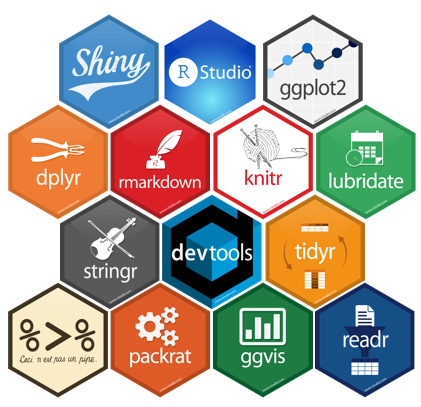
\includegraphics[width=0.9\linewidth]{plots01/rstudiopackages.jpeg}
%	\caption{}
	\label{fig:rstudiopackages}
\end{figure}

\begin{itemize}
\footnotesize	\item En los últimos años se han generado muchas herramientas para analizar, explorar, modelizar, comunicar y conectar los resultados del trabajo en R.
	\item De esta manera, podemos integrar el análisis de datos al flujo de trabajo mediante aplicaciones web, documentos (markdown o \LaTeX) o interfases con otros programas.
\end{itemize}
\end{multicols}

	
Links:
\begin{itemize}
\scriptsize	\item R: \url{https://cran.r-project.org/}
	\item RStudio: \url{https://posit.co/download/rstudio-desktop/}
	\item RStudio Cloud: \url{https://posit.cloud/}
\end{itemize}	
\end{frame}

\begin{frame}
\frametitle{Expresiones y asignaciones}
\begin{itemize}
	\item Expresión:  7 * 8 $\rightarrow$ R devuelve el resultado
	\item Asignación: X = 10 * 4
	\begin{itemize}
		\item R no devuelve el resultado
		\item el resultado queda guardado: ver en "Environment", arriba a la derecha
		\item si en la siguiente línea escribimos \textit{X}, el programa nos devuelve el resultado
		\item prestar atención a las mayúsculas y minúsculas 
		\item X = X + 10 ?
	\end{itemize}
	\item \onslide<2->{Asignaciones no son ecuaciones!}
	\item \onslide<3->{Comparadores: <, >, <=, >=, ==, !=}
	\item \onslide<4->{Operadores lógicos: AND (\&), OR (|), XOR (xor), NOT(!)}
\end{itemize}
\end{frame}

\begin{frame}
\frametitle{Funciones}
\begin{itemize}
	\item funciones simples: 
	\begin{itemize}
		\item $\sin$(pi), $\sin$(pi/2)
		\item $\exp(10)$ 
		\item 100 ** 2 
		\item $\log$(1)
		\item sec = 1:14
		\item seq(0,1,0.01)
		\item rnorm(100)
	\end{itemize}
	\item Composición de funciones: 
	\begin{itemize}
		\item mean(rnorm(100))
		\item exp(log(pi))
		\item plot(rnorm(100),type="l")
		\item plot(density(rnorm(10000)))
	\end{itemize}
\end{itemize}
\end{frame}

\begin{frame}
\frametitle{Vectores y matrices}
\begin{itemize}
	\item Vectores: 
	\begin{itemize}
		\item vec = vector("numeric",10)
		\item vec[i]: el i-ésimo número en el vector
		\item vec[4] = 5
	\end{itemize}
	\item Matrices:
	\begin{itemize}
		\item mat = matrix(0,nrow=3,ncol=3)
		\item mat[i,j] = valor correspondiente a la asignación de la fila "i" y la columna "j".
		\item mat [1,2] = 3
	\end{itemize}
\end{itemize}
\end{frame}

\begin{frame}
\frametitle{Loops - Estructuras de control}
\begin{itemize}
	\item \underline{For:} utilizado para ejecutar una serie de comandos \textit{n} veces. 
	\begin{itemize}
		\item Sintaxis: \textbf{for ( condición ) \{ acción \}}
		\onslide<2->{\item Ejemplo: for ( i in 1:10 ) \{ x = x + 1 \}
		\item Ejemplo: for ( i in 1$:$ length(vect) ) \{ x = x - 1 \}}
	\end{itemize}
  	\onslide<3->{\item \underline{ While:} utilizado para ejecutar una serie de comandos, mientras la condición sea cierta.
 	\begin{itemize}
 		\item Sintaxis: \textbf{while ( condición ) \{ acción \}}}
 		\onslide<4->{\item Ejemplo: while ( i < 10 )  \{ x = x*2 ; i= i + 1	\}}
 	\end{itemize}
 	\item \onslide<5->{\underline{if:} utilizado para ejecutar una serie de comandos, si la condición es cierta.
 	\begin{itemize}
 		\item Sintaxis: \textbf{if ( condición1 ) \{ acción1 \} else \{ acción2 \}}}
 		\onslide<6->{\item Ejemplo: if ( x < 1500 )  \{ x = x*2 \}
 		\\ else  \{ x = x * 2 /3 \}}
 	\end{itemize}
\end{itemize}
\end{frame}

\begin{frame}
	\frametitle{Escribir un modelo en R}
	\framesubtitle{¿Qué datos necesitamos?}
	Para escribir un modelo, necesitamos conocer:
	\begin{itemize}
		\item Parámetros del modelo.
		\item Variables del modelo.
		\item Manera en que se relacionan los parámetros y las variables (ecuaciones).
		\item Valores iniciales de las variables.
	\end{itemize}
\end{frame}

\begin{frame}
\frametitle{ejemplo 1: Ecuación logística}
\scriptsize
Esta ecuación la podemos escribir de la siguiente manera:
\begin{equation*}
q_{t+1}=Aq_{t}(1-q_t)
\end{equation*}

Entonces, para graficar la curva:
\begin{itemize}
	\item dar un valor al parámetro A (comenzar con \texttt{\textcolor{blue}{A = 2}})
	\item generar una secuencia de valores posibles para $q_t$ \\- sugerencia: \texttt{\textcolor{blue}{q=seq(0,1,0.001)}} -
	\item generar un valor de la función logística para cada valor de $q_t$: \texttt{\textcolor{blue}{logist[i]=A*q[i](1-q[i])}}
\end{itemize}
Ahora, para calcular el resultado a partir de un valor inicial:
\begin{itemize}
	\item creamos un vector de resultados, con 500 períodos: \texttt{\textcolor{blue}{result=vector("numeric",500)}}

	\item para el primer período, le imputamos un valor inicial igual a 0.3 \\\texttt{\textcolor{blue}{result[1]=0.3}}
	\item escribimos el loop, partiendo de la condición inicial\\
\texttt{\textcolor{blue}{for (i in 2:length(result)) \{result[i]=....................................\}}}
	\end{itemize}
\end{frame}

\begin{frame}
	\frametitle{Para graficar}
\begin{itemize}
	\item Utilizamos funciones: plot, lines, segments, points
	\item Al graficar \textbf{logist} y \textbf{q} respecto a \textbf{q}, tenemos el gráfico habitual de la ecuación logística.
	\item Ahora, utilizamos las funciones \textbf{segments} y \textbf{points} para representar la dinámica, a partir del valor del parámetro y de un valor inicial.
\end{itemize}	
\vspace{-0.4cm}
\begin{figure}
\centering
\includegraphics[width=0.23\linewidth,angle=270]{plots01/plot_a_2.eps}
\includegraphics[width=0.23\linewidth,angle=270]{plots01/plot_a_28.eps}
\includegraphics[width=0.23\linewidth,angle=270]{plots01/plot_a_34.eps}
\includegraphics[width=0.23\linewidth,angle=270]{plots01/plot_a_384.eps}
  %  \caption{Caption}
    \label{fig:my_label}
\end{figure}
\end{frame}

\begin{frame}{ciclos}
    \begin{figure}
        \centering
\includegraphics[width=0.3\linewidth,angle=270]{plots01/plot_2_ciclo.eps}
\includegraphics[width=0.3\linewidth,angle=270]{plots01/plot_4_ciclo.eps}
\includegraphics[width=0.3\linewidth,angle=270]{plots01/plot_3_ciclo.eps}
\includegraphics[width=0.3\linewidth,angle=270]{plots01/plot_caos.eps}
    %    \caption{Caption}
        \label{fig:my_label}
    \end{figure}
\end{frame}

\begin{frame}{Diagrama de bifurcación}
\vspace{-1cm}
\begin{figure}
    \centering
    \includegraphics[width=0.7\linewidth,angle=270]{plots01/bifurcacion.eps}
    %\caption{Caption}
    \label{fig:my_label}
\end{figure}
    
\end{frame}
	
	
\end{document}

